\begin{figure}
  \centering
  \begin{subfigure}[b]{0.45\textwidth}
    \centering
    
\includegraphics[width=\textwidth]{img/simi-stand-withpic.jpg}
    \caption{} % force the (a) to show up
    \label{fig:example-1}
  \end{subfigure}
  \begin{subfigure}[b]{0.45\textwidth}
    \centering
    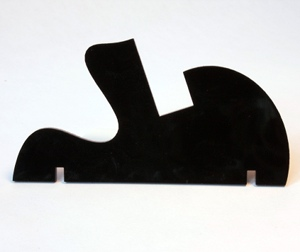
\includegraphics[width=\textwidth]{img/simi-stand-part.jpg}
    \caption{} % force the (b) to show up
    \label{fig:example-2}
  \end{subfigure}
  \caption[Picture frame stand]{A picture stand (\subref{fig:example-1})
    drawn and fabricated using SIMI. A single copy of the primary part
    is shown in (\subref{fig:example-2}). }
  \label{fig:simi-example}
\end{figure}
